\documentclass{article}

% Language setting
% Replace `english' with e.g. `spanish' to change the document language
\usepackage[spanish]{babel}

% Set page size and margins
% Replace `letterpaper' with `a4paper' for UK/EU standard size
\usepackage[letterpaper,top=2cm,bottom=2cm,left=3cm,right=3cm,marginparwidth=1.75cm]{geometry}

% Useful packages
\usepackage{amsmath}
\usepackage{graphicx}
\usepackage[colorlinks=true, allcolors=blue]{hyperref}
\usepackage{textgreek}
\usepackage{verbatim}
\usepackage{caption}
\usepackage{subcaption}
\usepackage{float}
\usepackage{array}
\usepackage{listings}
\usepackage{xcolor}
\usepackage{natbib}




\begin{document}

\definecolor{background}{rgb}{0.95,0.95,0.92}  % Light gray background color

\lstset{ 
  language=Python,                % the language of the code
  basicstyle=\ttfamily\small,     % the size of the fonts that are used for the code
  numbers=left,                   % where to put the line-numbers
  numberstyle=\tiny\color{gray},  % the style that is used for the line-numbers
  stepnumber=1,                   % the step between two line-numbers. If it's 1, each line will be numbered
  numbersep=5pt,                  % how far the line-numbers are from the code
  backgroundcolor=\color{white},  % choose the background color. You must add \usepackage{color}
  showspaces=false,               % show spaces adding particular underscores
  showstringspaces=false,         % underline spaces within strings
  showtabs=false,                 % show tabs within strings adding particular underscores
  frame=single,                   % adds a frame around the code
  rulecolor=\color{black},        % if not set, the frame-color may be changed on line-breaks within not black text (e.g. comments (green here))
  tabsize=2,                      % sets default tabsize to 2 spaces
  captionpos=b,                   % sets the caption-position to bottom
  breaklines=true,                % sets automatic line breaking
  breakatwhitespace=false,        % sets if automatic breaks should only happen at whitespace
  title=\lstname,                 % show the filename of files included with \lstinputlisting; also try caption instead of title
  keywordstyle=\color{blue},      % keyword style
  commentstyle=\color{gray},      % comment style, changed to magenta for better readability
  stringstyle=\color{red},        % string literal style
  escapeinside={\%*}{*)},         % if you want to add LaTeX within your code
  morekeywords={*,...}            % if you want to add more keywords to the set
}


\begin{titlepage}
\centering
{\bfseries\LARGE Universidad Politécnica de Valencia\par}
\vspace{1cm}
{\scshape\Large Escuela Técnica Superior de Ingeniería Informática\par}
\vspace{3cm}
{\scshape\Huge Lectura de llaves RFID-RC522 \par}
\vspace{3cm}
{\itshape\Large Proyecto Internet de las Cosas\par}
\vfill
{\Large Abel Haro Armero \par}
\vfill
{\Large Junio 2024 \par}
\date{}
\end{titlepage}



\tableofcontents

\newpage


\section{Introducción}

Este proyecto consiste en desarrollar un sistema de control de acceso utilizando tecnología RFID (lector RFID-RC522).
El sistema permitirá registrar usuarios y controlar su acceso mediante llaves y tarjetas RFID. 
Para el cambio de modo del lector, entre registro o acceso, se utilizará comunicación Bluetooth. 
Los usuarios registrados y los accesos se mantendrán en una base de datos accesible mediante una API REST dentro de un contenedor. 
Para la visualización se utilizará Ubidots.
Todo el proyecto se encuentra en un repositorio de GitHub \href{https://github.com/AbelHaro/Lectura-de-llaves-RFID-RC522}{Lectura de llaves RFID-RC522} \cite{abelharo2024lectura}.

\begin{figure}[H]
\centering
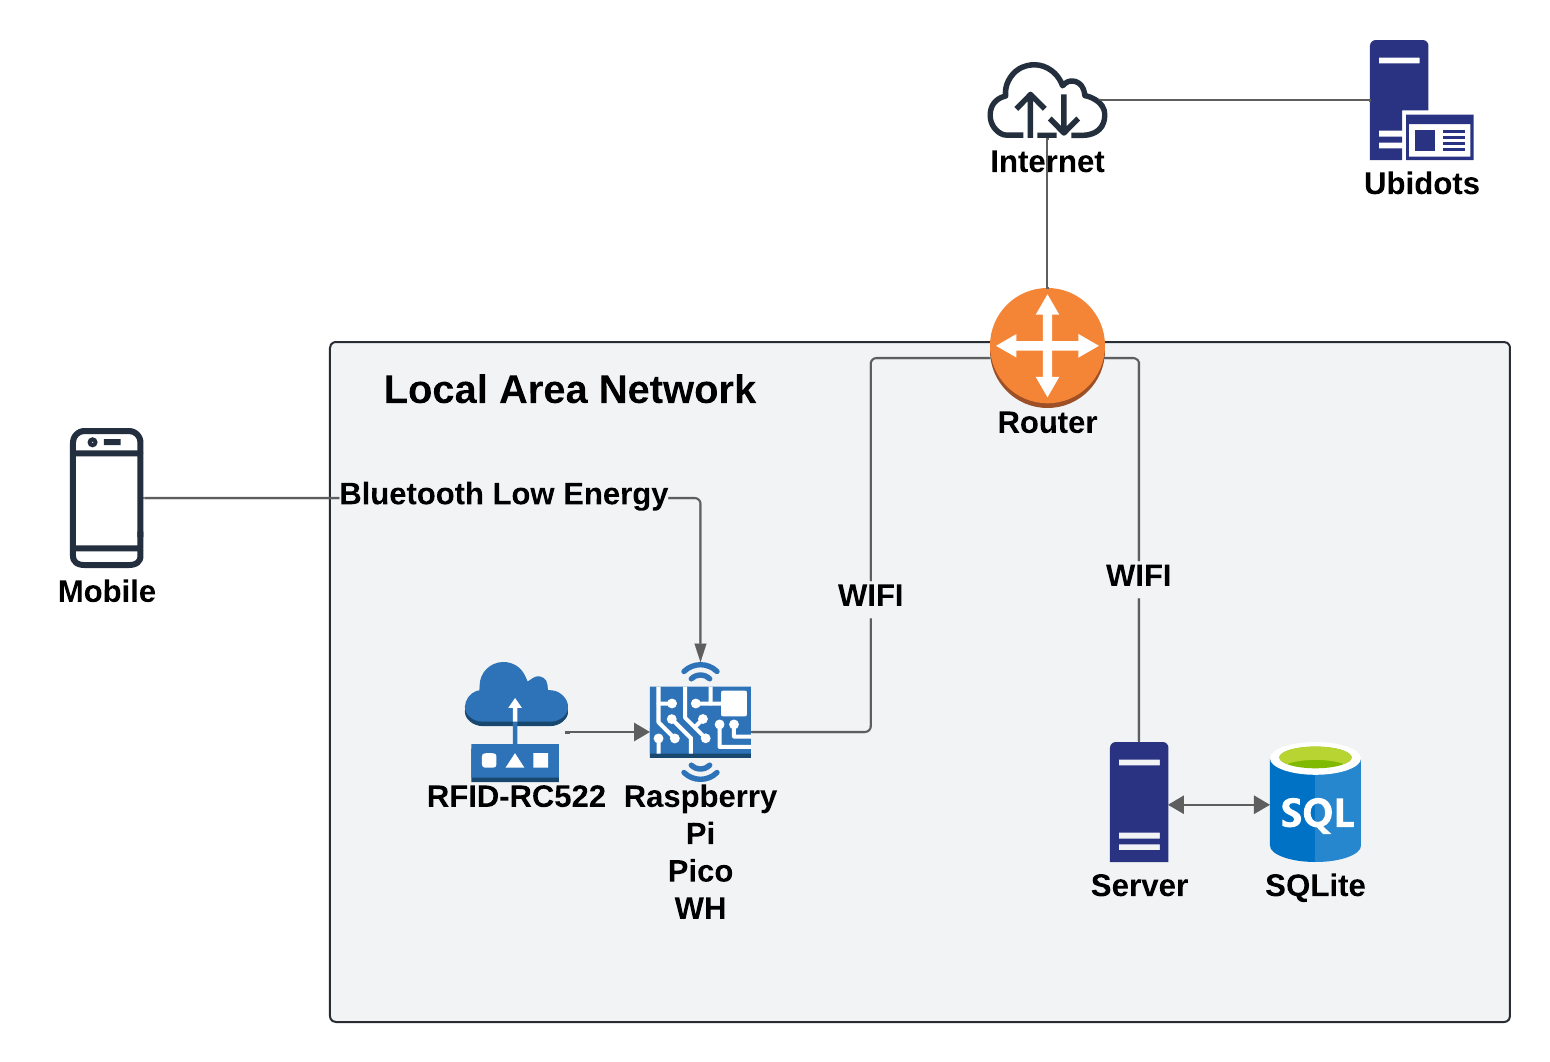
\includegraphics[width=0.9\linewidth]{../images/esquema_proyecto.png}
\caption{\label{fig:esquema red}Esquema del proyecto.}
\end{figure}

\section{Hardware utilizado}
Para el proyecto se ha utilizado el siguiente hardware:

\begin{figure}[H]
	\centering
	\begin{subfigure}[b]{0.45\textwidth}
		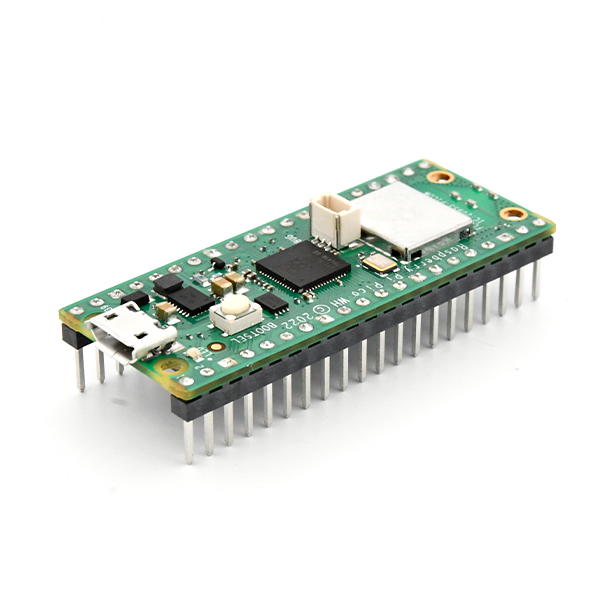
\includegraphics[width=\textwidth]{../images/picowh.png}
		\caption*{\href{https://www.raspberrypi.com/products/raspberry-pi-pico/}{Microcontrolador Raspberry Pi Pico WH}}
		\label{fig:picowh}
	\end{subfigure}
	\hfill
	\begin{subfigure}[b]{0.45\textwidth}
		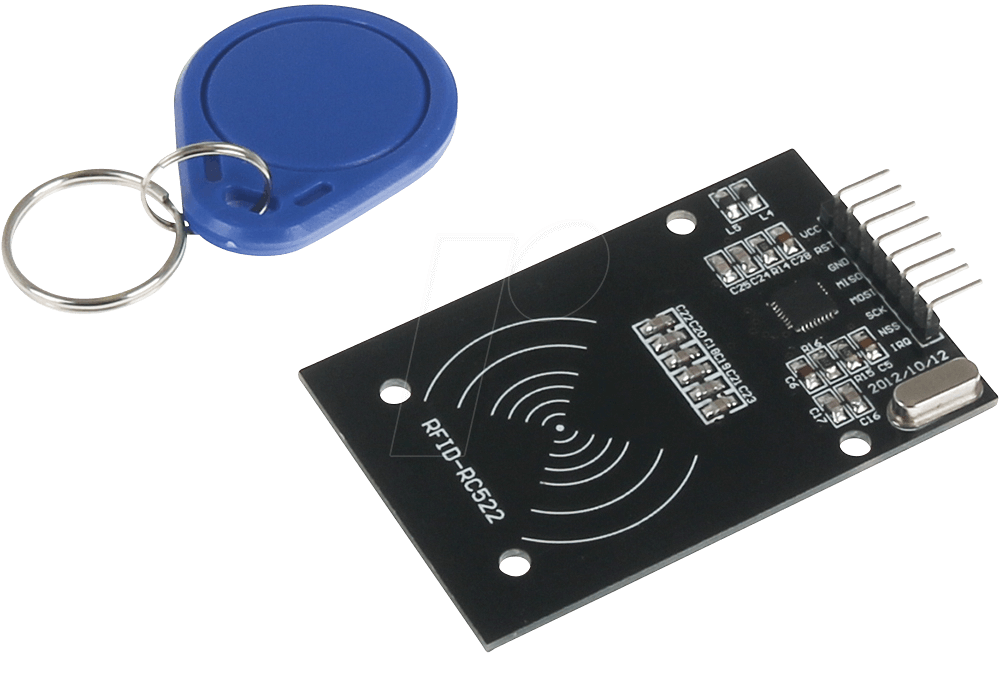
\includegraphics[width=\textwidth]{../images/mfrc522.png}
		\caption*{\href{https://www.keyestudio.com/products/keyestudio-mfrc522-rfid-s50-fudan-card-ic-card-module-with-spi-port-for-arduino-uno-r3-mega-2560-r3}{Lector de radiofrecuencia RFID-RC522}}
		\label{fig:MFRC522}
	\end{subfigure}
\end{figure}

\begin{figure}[H]
	\centering
	\begin{subfigure}[b]{0.45\textwidth}
		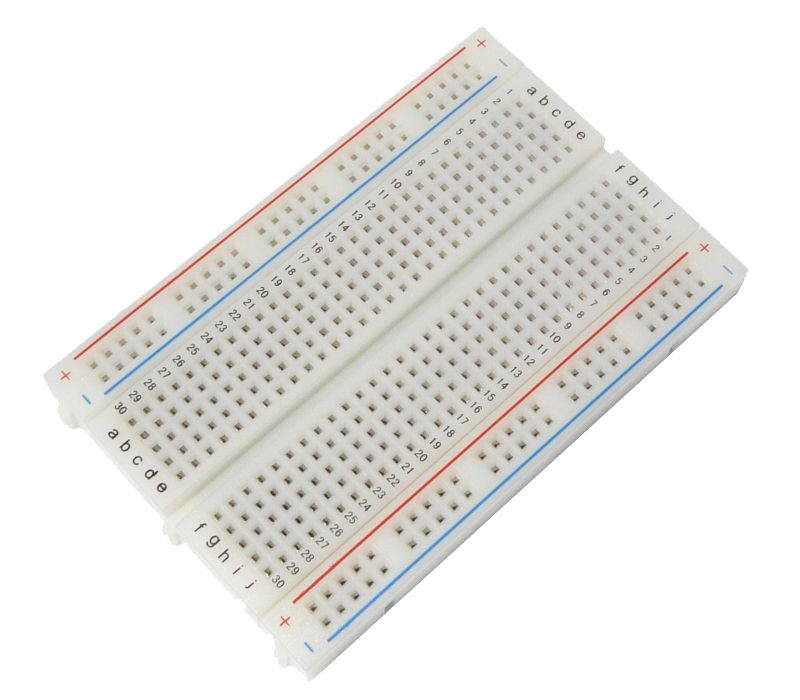
\includegraphics[width=\textwidth]{../images/protoboard.png}
		\caption*{Protoboard}
		\label{fig:protoboard}
	\end{subfigure}
	\hfill
	\begin{subfigure}[b]{0.45\textwidth}
		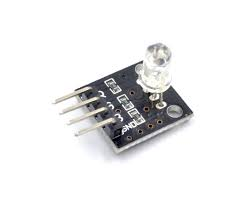
\includegraphics[width=\textwidth]{../images/led_tricolor.jpg}
		\caption*{Led tricolor KY-016 SP00}
		\label{fig:led tricolor}
	\end{subfigure}
\end{figure}

\begin{figure}[H]
	\centering
	\begin{subfigure}[b]{0.3\textwidth}
		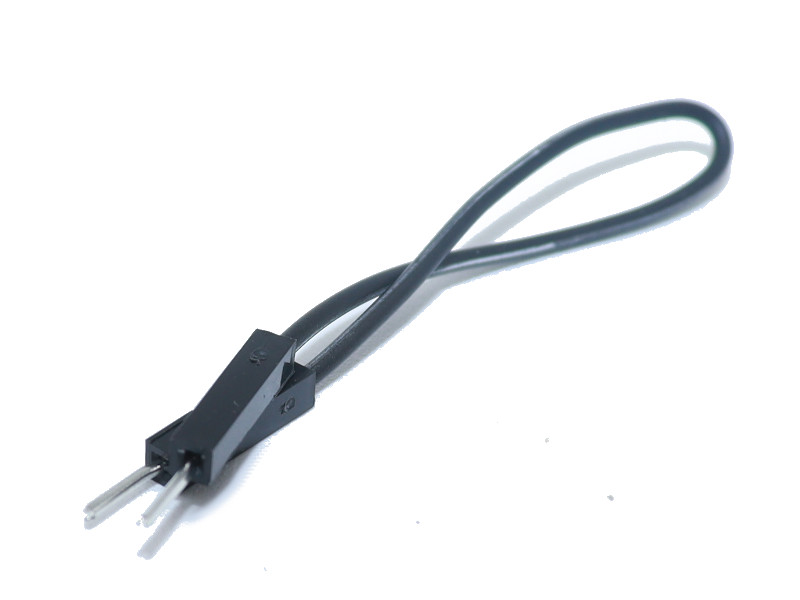
\includegraphics[width=\textwidth]{../images/cable_mm.jpg}
		\caption*{Cable Dupont Macho-Macho x3}
		\label{fig:cable mm}
	\end{subfigure}
	\hfill
	\begin{subfigure}[b]{0.3\textwidth}
		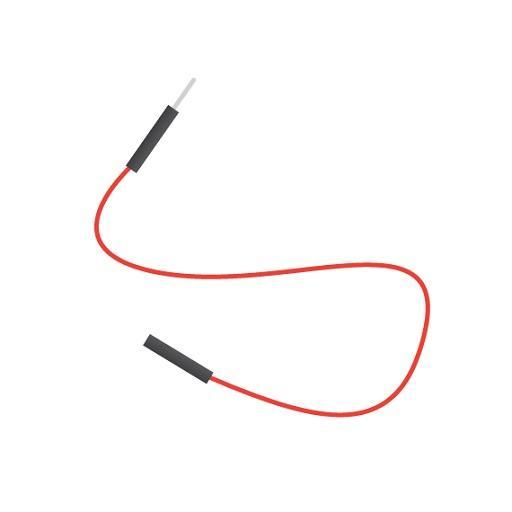
\includegraphics[width=\textwidth]{../images/cable_mh.jpg}
		\caption*{Cable Dupont Hembra-Macho x5}
		\label{fig:cable mh}
	\end{subfigure}
	\hfill
	\begin{subfigure}[b]{0.3\textwidth}
		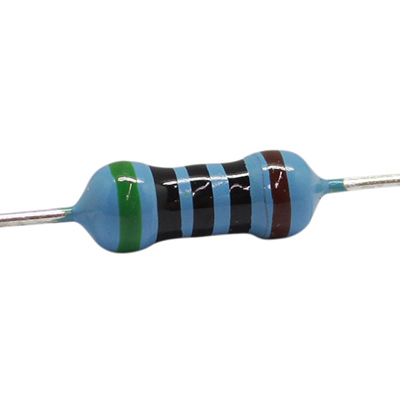
\includegraphics[width=\textwidth]{../images/resistencia.jpg}
		\caption*{Resistencia de 500\textOmega\ x2}
		\label{fig:resistencia}
	\end{subfigure}
\end{figure}


\section{Software utilizado}
Para la realización del proyecto se ha utilizado el siguiente software.
\subsection{Microcontrolador}
Como lenguaje de programación para el microcontrolador Raspberry Pi Pico WH se ha utilizado Micropython.
Para establecer y gestionar la comunicación Bluetooth en el microcontrolador se hizo uso de las \href{https://github.com/micropython/micropython/tree/master/examples/bluetooth}{bibliotecas BLE} (Bluetooth Low Energy)\cite{micropythonBluetoothExamples}.
Para el dispositivo móvil se utilizó la aplicación \href{https://play.google.com/store/apps/details?id=de.kai_morich.serial_usb_terminal&pcampaignid=web_share}{Serial Bluetooth Terminal}\cite{sam2023ble} disponible en Play Store. Para la lectura de llaves y tarjetas basadas en radiofrecuencia se utilizó la \href{https://github.com/danjperron/micropython-mfrc522/blob/master/mfrc522.py}{bibilioteca MFRC522} \cite{danjperron2022mfrc522}.
En la comunicación con el servidor se implementó una API REST que permite el envío y recepción de datos de manera estructurada. Por último, se hizo uso de la librería estándar machine para encender y apagar LEDs.

\subsection{Servidor}
En la implementación del servidor se hace uso de un contenedor Docker con la imagen base de Ubuntu. 
A la imagen se le instala Python junto con el paquete Flask para gestionar la lógica del servidor mediante solicitudes HTTP. 
Para la persistencia de datos se emplea un volumen de Docker junto con una base de datos SQLite.
Para el desarrollo del servidor se modifica el código de la \href{https://pmanzoni.notion.site/LAB-6-REST-d487dab1b7e24d56b31d8e552a480888}{práctica 6 - REST} \cite{manzoni2024lab6}.


\subsection{Ubidots}
Para la plataforma de visualización se ha utilizado \href{https://stem.ubidots.com/}{Ubidots} mediante una cuenta STEM. Ubidots permite la visualización de datos en tiempo real y un envío de 1 req/s.

\section{Pasos para realizar el proyecto}
Para la realización del proyecto se deben seguir los siguientes pasos.
\subsection{Paso 1: Preintstalación de software necesario}
\textbf{Instalaciones de aplicaciones en el servidor:}
\begin{enumerate}
    \item Instalar \href{https://thonny.org/}{Thonny}.
    \item Instalar \href{https://code.visualstudio.com/download}{Visual Studio Code}.
    \item Instalar \href{https://docs.docker.com/get-docker/}{Docker}.
    \item Instalar \href{https://kinsta.com/es/base-de-conocimiento/instalar-python/}{intérprete de Python}.
\end{enumerate}


\textbf{Instalación de archivos en la Raspberry Pi Pico WH:}
\begin{enumerate}
	\item Instalar firmware de MicroPython:
		\begin{enumerate}
			\item Introducir el USB en el ordenador mientras se aprieta el botón BOOTSEL.
			\item Abrir Thonny y realizar los siguientes pasos:
			\begin{figure}[H]
			\centering
			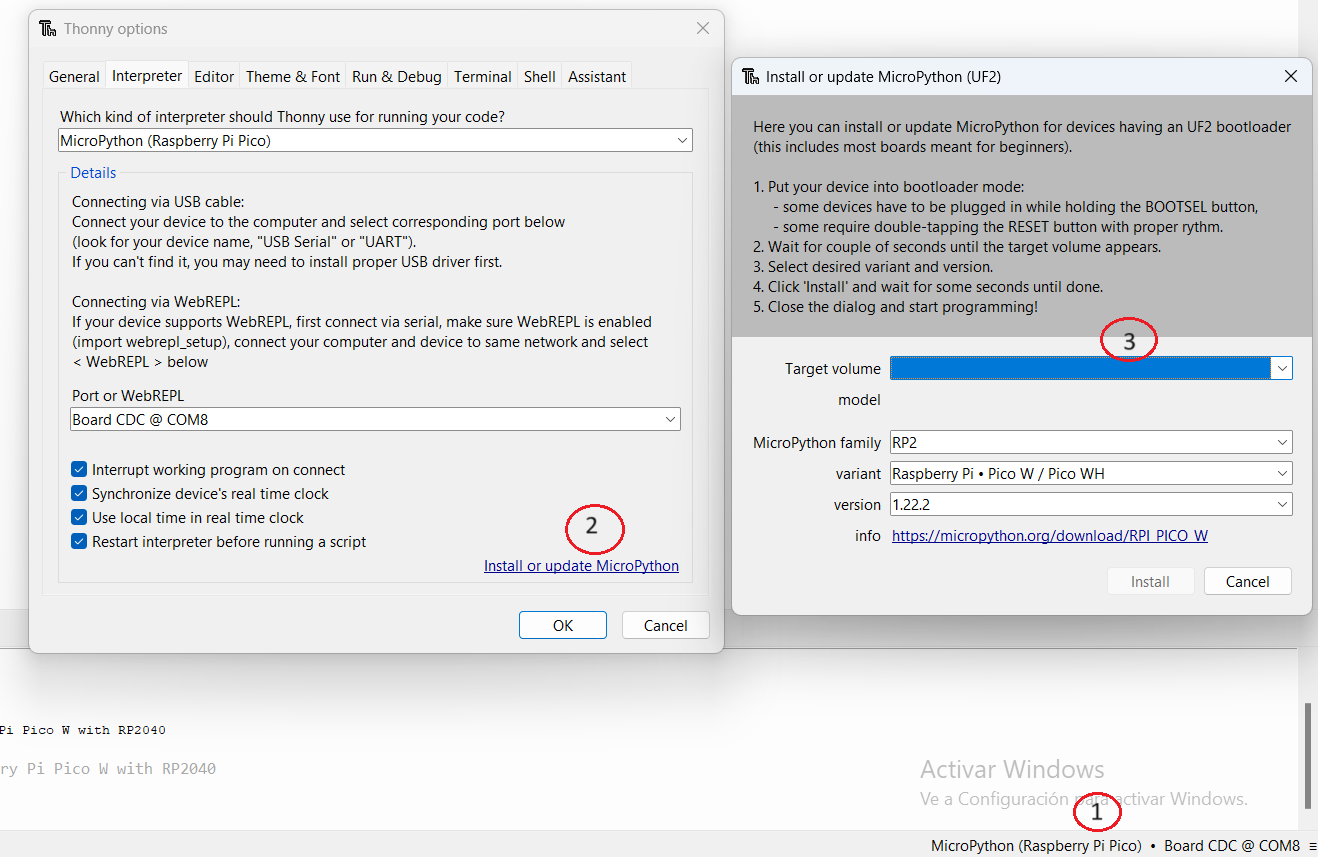
\includegraphics[width=0.8\linewidth]{../images/instalacion_firmware.png}
			\caption{\label{fig:instalación firmware}Pasos para la instalación del firmware.}
			\end{figure}
		\end{enumerate}
			\item Copiar el contenido de la carpeta \texttt{``microcontrolador''} del proyecto en la Raspberry Pi Pico WH.
			\item Configurar las variables \texttt{``ssid''} y \texttt{``password''} dentro del archivo \texttt{``microcontrolador/wifi\_connect.py''} con el \texttt{ssid} y \texttt{password} de tu red.
\end{enumerate}

\textbf{Resgistro y configuración de Ubidots:}
\begin{enumerate}
	\item Crear una cuenta en \href{https://stem.ubidots.com/}{Ubidots Stem}.
	\item Crear un nuevo dispositivo.
	\begin{figure}[H]
		\centering
		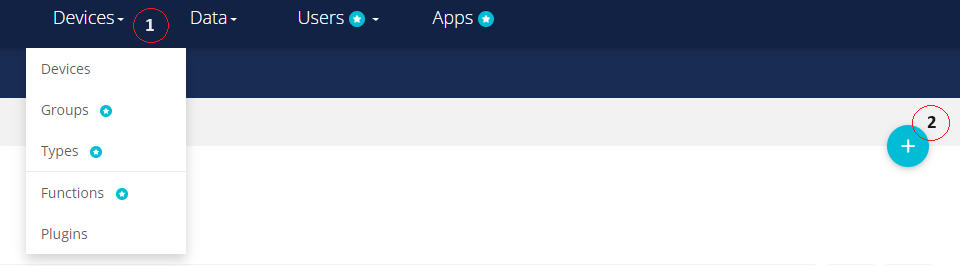
\includegraphics[width=0.7\linewidth]{../images/ubidots_create_device_1.png}
		\caption{\label{fig:ubidots_create_device_1}Creación de un nuevo dispositivo en Ubidots.}
	\end{figure}
	\item Añadir el nombre del dispositivo a la variable  \texttt{``DISPOSITIVE\_NAME''} dentro del archivo \texttt{``api/ubidots\_conf.py''}.
	\item Dentro del dispositivo crear dos \texttt{``raw variable''}, una para el registro de usuarios \texttt{``add\_user\_register''} y otra para el registro de accesos de los usarios \texttt{``add\_time\_registry''}.
	\begin{figure}[H]
		\centering
		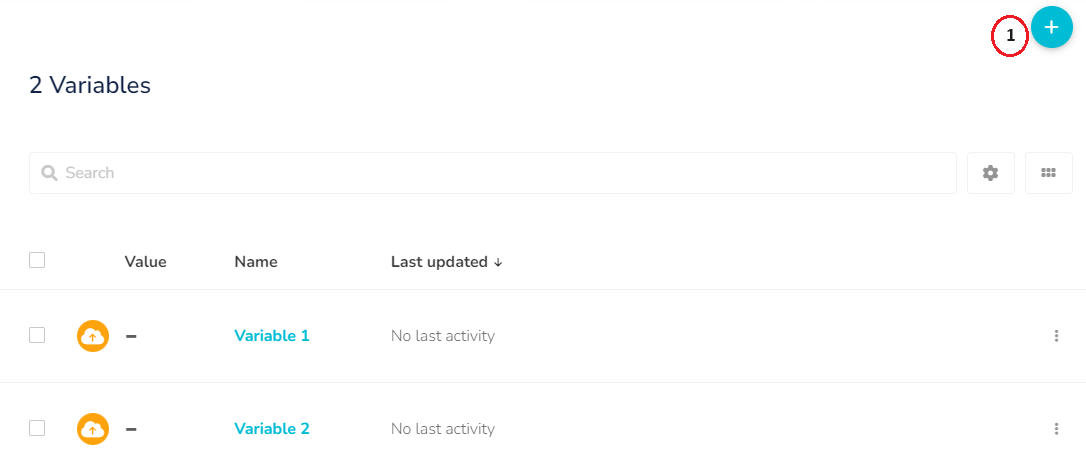
\includegraphics[width=0.7\linewidth]{../images/ubidots_create_variable.png}
		\caption{\label{fig:ubidots_create_variable_1}Creación de una variable en Ubidots.}
	\end{figure}
	\item Obteber el token de la API.
		\begin{figure}[H]
			\centering
			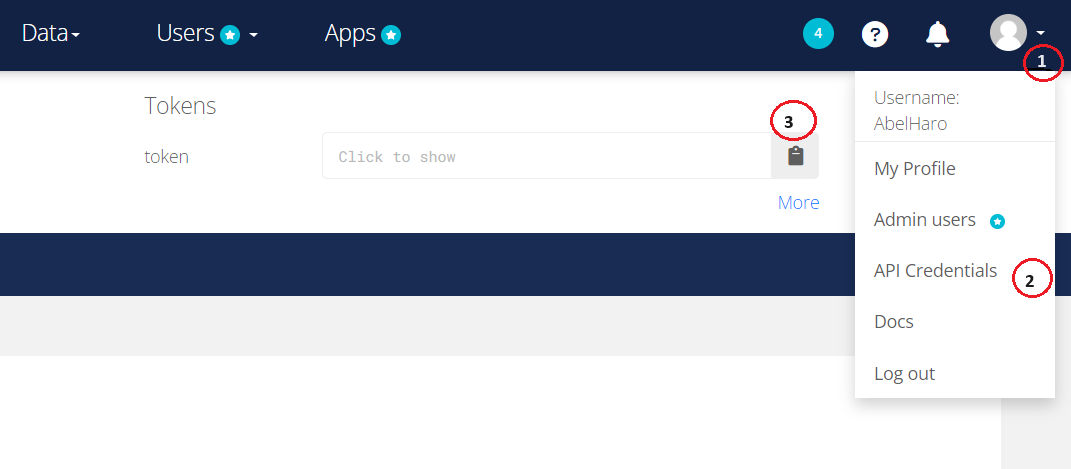
\includegraphics[width=0.7\linewidth]{../images/ubidots_obtener_token.png}
			\caption{\label{fig:ubidots_obtener_token}Obtención del token de la API en Ubidots.}
		\end{figure}
	\item Copiar el token de la API a la variable \texttt{``TOKEN\_UBIDOTS''} dentro del archivo \texttt{``api/ubidots\_conf.py''}.
\end{enumerate}

\subsection{Paso 2: Montaje circuito}
Para el montaje del circuito se ha seguido como referencia el siguiente vídeo \href{https://www.youtube.com/watch?v=bvn_o39uXac}{`RFID RC522 con Raspberry Pi Pico y Códigos en MicroPython para simple Control de Acceso'} \cite{computadoras2022rfid}.\\
Conectar el lector RFID-RC522 a la Raspberry Pi Pico WH siguiendo la siguiente tabla:

\begin{center}
	\begin{tabular}{|c|c|}
		\hline
		\textbf{Lector RFID-RC522} & \textbf{Raspberry Pi Pico WH} \\
		\hline
		VCC & 3.3V \\
		\hline
		RST & GP0 \\
		\hline
		GND & GND \\
		\hline
		IRQ & No conectado \\
		\hline
		MISO & GP4 \\
		\hline
		MOSI & GP3 \\
		\hline
		SCK & GP2 \\
		\hline
		SDA & GP1 \\
		\hline
	\end{tabular}
	\captionof{table}{Conexiones entre el lector RFID-RC522 y la Raspberry Pi Pico WH.}
\end{center}

\vspace{0.3cm}

Conectar el LED tricolor KY-016 SP00 a la Raspberry Pi Pico WH siguiendo la siguiente tabla:
\begin{center}
	\begin{tabular}{|c|c|}
		\hline
		\textbf{KY-016 SP00} & \textbf{Raspberry Pi Pico WH} \\
		\hline
		R & GP13 \\
		\hline
		G & GP12 \\
		\hline
		B & No conectado \\
		\hline
		- & GND \\
		\hline
	\end{tabular}
	\captionof{table}{Conexiones entre el LED tricolor KY-016 SP00 y la Raspberry Pi Pico WH.}
\end{center}



El montaje del circuito debe quedar como se muestra en la siguiente figura:
\begin{figure}[H]
	\centering
	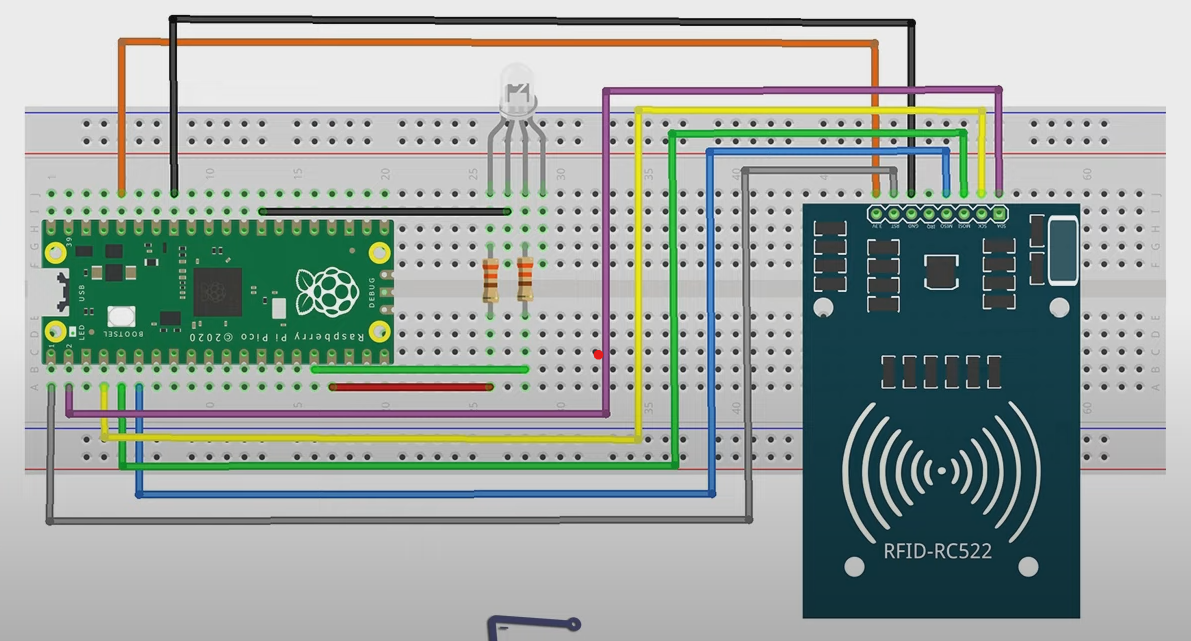
\includegraphics[width=1\linewidth]{../images/esquema_de_conexionado.png}
	\caption{\label{fig:circuito}Esquema de conexionado del proyecto.}
\end{figure}

\subsection{Paso 3: Ejecución del proyecto}
Para ejecutar el proyecto se deben seguir los siguientes pasos:
\begin{enumerate}
	\item Conectar la Raspberry Pi Pico WH al ordenador.
	\item Abrir Thonny y ejecutar el archivo \texttt{``microcontrolador/main.py''} en la Raspberry Pi Pico WH.
	\item Arrancar el daemon de Docker.
	\item Ejecutar el archivo \texttt{``build.bat''} en el servidor.
	\item Abrir Ubidots y visualizar los datos.
	\item Realizar pruebas de registro y acceso.
\end{enumerate}

\section{Programación del proyecto}
En esta sección se muestra en detalle el código de los archivos de los archivos principales del proyecto.

\subsection{Microcontrolador}
\subsubsection{main.py}
Este archivo es el principal del microcontrolador.
Contiene la configuración de la comunicación Bluetooth y la función \texttt{``on\_rx(data)''} donde se recibe el mensaje bluetooth para el cambio de modo de lectura.
En la función \texttt{``main()''} se llama a la función \texttt{``wifi.connect()''} para conectar a la red WiFi y se inicia el bucle principal del programa.
En el bucle se llama a la función \texttt{``sensor.read\_sensor()''} y recibe el uid de la llave o tarjeta RFID. 
Si el modo es de registro se llama a la función \texttt{``sender.add\_user\_register(uid)''} y si es el modo de registro de entrada se llama a la función \texttt{``sensor.add\_time\_registry(uid)''}.
Por último se llama a la función \texttt{``led.blink\_led(response[`api\_status'])''} para encender el led tricolor en función de la respuesta de la API.

\begin{lstlisting}
	import bluetooth  # Bluetooth module
	from ble.ble_simple_peripheral import BLESimplePeripheral  # BLE module
	import time
	import wifi_connect as wifi
	import data_sending_api as sender
	import sensor
	import led_control as led
	import ubidots
	
	# Initialize Bluetooth Low Energy (BLE) interface and Simple Peripheral
	ble = bluetooth.BLE()
	sp = BLESimplePeripheral(ble, name="Pico WH")
	
	# Default mode for RFID sensor operation
	MODE = 'ADD_USER_REGISTER'  # Default mode is to add user registration
	
	def on_rx(data):
		"""
		Callback function for receiving data from BLE.
	
		Parameters:
			data (bytes): Received data as bytes.
	
		Global Variables Modified:
			MODE (str): Updated mode based on received data.
		"""
		global MODE  # Access global variable MODE within the function
		print("Data received:", data)
	
		# Update mode based on received data
		if data == b'ADD_USER_REGISTER\r\n':
			MODE = 'ADD_USER_REGISTER'
		elif data == b'ADD_TIME_REGISTRY\r\n':
			MODE = 'ADD_TIME_REGISTRY'
	
	
	if __name__ == '__main__':
		# Connect to WiFi
		wifi.connect()
	
		try:
			if sp.is_connected():
				sp.on_write(on_rx)  # Register callback for BLE data reception
				
			while True:
				# Read UID from sensor
				uid = sensor.read_sensor()
				
				# Determine mode and call appropriate API
				if MODE == 'ADD_USER_REGISTER':
					response = sender.add_user_register(uid)  # Call API to add user registration
				elif MODE == 'ADD_TIME_REGISTRY':
					response = sender.add_time_registry(uid)  # Call API to add time registry
				else:
					print('Error: Invalid mode')
					raise Exception('Invalid mode detected')  # Raise an exception for invalid mode
				
				# Blink LED based on API response status
				led.blink_led(response['api_status'])
				time.sleep(1)
		except KeyboardInterrupt:
			print('Programa abortado con CTRL+C desde main.py')  # Handle keyboard interrupt
	\end{lstlisting}
	\captionof{figure}{Código del archivo \texttt{``microcontrolador/main.py''} del microcontrolador.}
	
\subsubsection{sensor.py}
Este archivo contiene la función \texttt{``read\_sensor()''} que lee el sensor RFID y devuelve el uid de la llave o tarjeta RFID leída.
\begin{lstlisting}
from lib.mfrc522.mfrc522 import MFRC522  # RFID reader module
import time  # Time-related functions
import data_sending_api as sender  # Custom API module for data sending

def read_sensor() -> str:
    """
    Function to read RFID sensor and perform actions based on the received data.

    Returns:
        str: UID from card or key readed.
    """
    # Initialize the MFRC522 RFID reader
    lector = MFRC522(spi_id=0, sck=2, miso=4, mosi=3, cs=1, rst=0)

    print("RFID sensor active...\n")

    try:
        while True:
            lector.init()  # Initialize the RFID reader
            (stat, tag_type) = lector.request(lector.REQIDL)  # Request tag detection

            if stat == lector.OK:
                (stat, uid) = lector.SelectTagSN()  # Select detected tag
                if stat == lector.OK:
                    # Convert UID bytes to integer for identification
                    identificador = int.from_bytes(bytes(uid), "little", False)
                    print("UID: " + str(identificador))  # Print detected UID

                    return str(identificador)  # Convert UID to string
                
            time.sleep(1)  # Sleep for 1 second between iterations

    except KeyboardInterrupt:
        print("Program terminated with CTRL+C from sensor.py")  # Handle keyboard interrupt
\end{lstlisting}
\captionof{figure}{Código del archivo \texttt{``microcontrolador/sensor.py''} del microcontrolador.}

\subsubsection{data\_sending\_api.py}
Este archivo contiene las funciones para enviar datos mediante la API REST del servidor.
Se tienen las funciones \texttt{``add\_user\_register(uid)''} y \texttt{``add\_time\_registry(uid)''} para enviar los datos de registro de usuario y de acceso respectivamente.

\begin{lstlisting}
import time  # Standard Python time module
import ujson  # Module for handling JSON data
import urequests as requests  # Module for making HTTP requests (alias for urequests)

URL = 'http://192.168.1.2:8888/api/'
URL_add_user_register = URL + 'user_register/add'
URL_add_time_registry = URL + 'time_registry/add'
URL_get_user_registered_by_uid = URL + 'user_register'

def get_local_time() -> str:
    """
    Returns the timestamp formatted.
    """
    local_time = time.localtime()
    formatted_time = "{:04d}-{:02d}-{:02d} {:02d}:{:02d}:{:02d}".format(
    local_time[0],  # year
    local_time[1],  # month
    local_time[2],  # day
    local_time[3],  # hour
    local_time[4],  # minute
    local_time[5]   # second
    )
    return str(formatted_time)

def add_user_register(uid):
    """
    Adds the user to the database using a POST request.
    
    Parameters:
        uid (str): The UID (Unique ID) of the user to be registered.
    
    Returns:
        dict: A dictionary containing the response message from the server.
    """
     
    data_sending = {
        "UID": uid,
        "user_creation_tstamp": get_local_time()
    }
    
    response = requests.post(URL_add_user_register, headers={'Content-Type': 'application/json'}, data=ujson.dumps(data_sending))
    return ujson.loads(response.content)
    
def add_time_registry(uid):
    """
    Adds the time registry to the database using a POST request.
    
    Parameters:
        uid (str): The UID (Unique ID) of the user to be registered.
    
    Returns:
        dict: A dictionary containing the response message from the server.
    """
    data_sending = {
        "UID": uid,
        "user_registry_tstamp": get_local_time()
    }
    
    response = requests.post(URL_add_time_registry, headers={'Content-Type': 'application/json'}, data=ujson.dumps(data_sending))
    return ujson.loads(response.content)

def get_user_registered_by_uid(uid):
    """
    Retrieves user registration details from the server based on UID using a GET request.
    
    Parameters:
        uid (str): The UID (Unique ID) of the user to be registered.
    
    Returns:
        dict: A dictionary containing the response message from the server.
    """
    response = requests.get(URL_get_user_registered_by_uid + '/%s'.format(uid))
    return ujson.loads(response.content)
\end{lstlisting}
\captionof{figure}{Código del archivo \texttt{``microcontrolador/data\_sending\_api.py''} del microcontrolador.}

\subsection{Servidor}
\subsubsection{api.py}
Este archivo contiene la API REST del servidor.
Contiene funciones para conectarse a la base de datos, añadir usuarios y registros de acceso, recuperar usuarios y registros de acceso mediante el UID y enviar el registro de usarios y accesos a Ubidots.
Para ello se muestran solo las funciones para el registro de usuarios \texttt{``insert\_user\_register()''}, \texttt{``get\_user\_register\_by\_uid(uid)''} y \texttt{``add\_user\_ubidots(uid)''} en la siguiente figura.

\begin{lstlisting}
import sqlite3
from flask import Flask, request, jsonify
import requests
from api.ubidots_conf import URL_UBIDOTS, TOKEN_UBIDOTS

...

def insert_user_register(user):
    """
    Inserts a new user registration record into the 'user_register' table and send it to Ubidots.

    Parameters:
        user (dict): Dictionary containing user information with keys:
                     - 'UID': Unique ID of the user.
                     - 'user_creation_tstamp': Timestamp of user creation.

    Returns:
        dict: Dictionary containing the status of the operation and error message (if any).
              Keys:
              - 'api_status': Boolean indicating the success of the operation.
              - 'error': Error message if an error occurred during the operation.
              - 'ubidots_status': HTTP status code of the request to Ubidots.
              - 'UID': Unique ID of the user.
              - 'user_creation_tstamp': Timestamp of user creation.
    """
    inserted_user = {'api_status': False, 'error': None, 'ubidots_status': False, 'UID': None, 'user_creation_tstamp': None}
    try:
        conn = connect_to_db()
        conn.row_factory = sqlite3.Row
        cur = conn.cursor()
        cur.execute("SELECT * FROM user_register WHERE UID = ?", (user['UID'],))
        rows = cur.fetchall()
        if len(rows) > 0:
            inserted_user['error'] = "User already exists"
            return inserted_user
        
        cur.execute("INSERT INTO user_register (UID, user_creation_tstamp) VALUES (?, ?)",
                    (user['UID'], user['user_creation_tstamp']) )
        conn.commit()
        inserted_user.update(get_user_register_by_uid(user['UID']))
        ubidots_status = add_user_ubidots(user['UID'])
        if ubidots_status == 200:
            inserted_user['api_status'] = True
        else :
            inserted_user['error'] = "Error adding user to Ubidots"
            
        inserted_user['ubidots_status'] = ubidots_status
    except:
        conn.rollback()
    finally:
        conn.close()
    return inserted_user

	def get_user_register_by_uid(uid):
    """
    Retrieves a user record from the 'user_register' table based on the provided UID.

    Parameters:
        uid (str): The UID (Unique ID) of the user to retrieve.

    Returns:
        dict: A dictionary representing the user record if found, otherwise an empty dictionary.
              The dictionary contains keys 'UID' and 'user_creation_tstamp' with corresponding values.
    """
    user = {}
    try:
        conn = connect_to_db()
        conn.row_factory = sqlite3.Row
        cur = conn.cursor()
        cur.execute("SELECT * FROM user_register WHERE UID = ?", (uid,))
        rows = cur.fetchall()

        # convert row objects to dictionary
        for i in rows:
            user["UID"]  = i["UID"]
            user["user_creation_tstamp"]  = i["user_creation_tstamp"]
            
    except:
        user = {}
    return user

	def add_user_ubidots(uid):
    """
    Sends an HTTP POST request to Ubidots API to add a user registration.

    Parameters:
        uid (str): The UID (User ID) of the user to register.

    Returns:
        int: HTTP status code of the request.
    """
    data = {
        'add_user_register': {
            'value': 1,
            'context': {
                'UID': uid
            }
        }
    }
    request = requests.post(
        URL_UBIDOTS,
        headers={'X-Auth-Token': TOKEN_UBIDOTS, 'Content-Type': 'application/json'},
        json=data
    )
    return request.status_code
	
	@app.route('/api/user_register/<uid>', methods=['GET'])
    def api_get_user_register_by_id(uid):
        return jsonify(get_user_register_by_uid(uid))
    
    @app.route('/api/user_register/add', methods=['POST'])
    def api_add_user_register():
        user = request.get_json()
        return jsonify(insert_user_register(user))

	app.run(host="0.0.0.0")
\end{lstlisting}
\captionof{figure}{Código del archivo \texttt{``api/api.py''} del servidor.}

\subsubsection{initdb.py}
Este archivo contiene la inicialización de la base de datos.
Para ello crea el directorio \texttt{``database''} si no existe y el archivo \texttt{``database.db''} si no existe.
Crea las tablas \texttt{``user\_register''} y \texttt{``time\_registry''} si no existen.

\begin{table}[H]
	\centering
	\begin{tabular}{|l|l|l|}
	\hline
	\textbf{Nombre columna} & \textbf{Tipo de dato} & \textbf{Restricciones} \\ \hline
	\texttt{UID} & \texttt{TEXT} & \texttt{PRIMARY KEY, NOT NULL} \\ \hline
	\texttt{user\_creation\_tstamp} & \texttt{TEXT} & \texttt{NOT NULL} \\ \hline
	\end{tabular}
	\caption{Tabla \texttt{user\_register} esquema.}
	\end{table}

\begin{table}[H]
	\centering
	\begin{tabular}{|l|l|p{8cm}|}
	\hline
	\textbf{Nombre columna} & \textbf{Tipo de dato} & \textbf{Restricciones} \\ \hline
	\texttt{id} & \texttt{INTEGER} & \texttt{PRIMARY KEY AUTOINCREMENT} \\ \hline
	\texttt{user\_registry\_tstamp} & \texttt{TEXT} & \texttt{NOT NULL} \\ \hline
	\texttt{UID} & \texttt{TEXT} & \texttt{NOT NULL, REFERENCES user\_register(UID)} \\ \hline
	\end{tabular}
	\caption{Tabla \texttt{time\_registry} esquema.}
	\end{table}

\begin{lstlisting}
import sqlite3
import os

if __name__ == '__main__':
    try:
        # Create the directory if it doesn't exist
        os.makedirs('database', exist_ok=True)
        print("Database directory created successfully.")

        # Create the database file if it doesn't exist
        open('database/database.db', 'a').close()
        print("Database file created successfully.")

        # Establish connection to the database
        conn = sqlite3.connect('database/database.db')
        print("Connection to the database established successfully.")

        # Create user_register table
        conn.execute('''
                    CREATE TABLE IF NOT EXISTS user_register (
                        UID    TEXT PRIMARY KEY NOT NULL,
                        user_creation_tstamp TEXT NOT NULL
                    )
        ''')
        print("Table 'user_register' created successfully.")

        # Create time_registry table
        conn.execute('''
                    CREATE TABLE IF NOT EXISTS time_registry (
                        id INTEGER PRIMARY KEY AUTOINCREMENT,
                        user_registry_tstamp TEXT NOT NULL,
                        UID TEXT NOT NULL REFERENCES user_register(UID)
                    )
         ''')

        print("Table 'time_registry' created successfully.")

        # Commit changes
        conn.commit()
        print("Changes committed successfully.")
    except Exception as e:
        print(e)
        print("Table creation failed")
    finally:
        conn.close()

\end{lstlisting}
\captionof{figure}{Código del archivo \texttt{``api/initdb.py''} del servidor.}

\subsubsection{build.bat, Dockerfile y start.sh}
Estos archivos son necesarios para la creación del contenedor Docker del servidor.
El archivo \texttt{``build.bat''} contiene los comandos para construir la imagen e iniciar el contenedor.
El archivo \texttt{``api/Dockerfile''} contiene las instrucciones para construir la imagen del contenedor.
El archivo \texttt{``api/start.sh''} contiene las instrucciones para inicializar la base de datos y ejecutar la API.


\begin{lstlisting}
	REM Change directory to the location of the Dockerfile
	cd ./api
	
	REM Build Docker image
	docker build -t server_rfid .
	
	REM Run Docker container
	docker run --rm -it -v database:/home/database -p 8888:5000 --name server_rfid server_rfid	
\end{lstlisting}
\captionof{figure}{Código del archivo \texttt{``build.bat''} del servidor.}

\begin{lstlisting}
FROM ubuntu

# Instalar Python 3 y Flask
RUN apt update
RUN apt install python3 python3-pip -y
RUN apt install python3-flask -y
RUN apt install python3-requests -y

# Establecer el directorio de trabajo y copiar los archivos
WORKDIR /home/
COPY initdb.py .
COPY api.py .
COPY start.sh .
COPY ubidots.py .

# Dar permisos para ejecutar el script
RUN chmod +x start.sh

# Exponer el puerto
EXPOSE 5000

# Ejecutar los scripts
CMD ["./start.sh"]

\end{lstlisting}
\captionof{figure}{Código del archivo \texttt{``api/Dockerfile''} del servidor.}

\begin{lstlisting}
	#!/bin/sh

# Check if the database directory exists, if not, create it (Only for the first run)
if [ ! -d "database" ]; then
    mkdir database
fi

# Initialize the database
python3 initdb.py

# Start the API
python3 api.py
\end{lstlisting}
\captionof{figure}{Código del archivo \texttt{``api/start.sh''} del servidor.}

\subsubsection{ubidots\_conf.py}
Este archivo contiene la configuración de Ubidots.
Contiene la URL de Ubidots, el dispositivo y el token de la API.
\begin{lstlisting}
DISPOSITIVE_NAME = '' # Device name in Ubidots
URL_UBIDOTS = f'http://industrial.api.ubidots.com/api/v1.6/devices/{DISPOSITIVE_NAME}/'
TOKEN_UBIDOTS = '' # Token of the API
\end{lstlisting}
\captionof{figure}{Código del archivo \texttt{``api/ubidots\_conf.py''} del servidor.}

\section{Problemas encontrados}
En los siguientes apartados se describen los problemas encontrados durante la realización del proyecto y las soluciones propuestas:
\subsection{Problema 1: Dirección estática del servidor} 
Para poder acceder al servidor desde la Raspberry Pi Pico WH siempre de la misma manera sin tener que modificar el código se debe tener una dirección IP estática en el servidor. Para ello se debe configurar la dirección IP estática accediendo a la configuración del router.
Se accede mediante un navegador web a la dirección IP del router en mi caso 192.168.1.1 y se introduce el usuario \texttt{``admin''} y la contraseña. Una vez dentro se busca la opción de configuración avanzada para acceder al servidor DHCP y se asigna una dirección IP estática al servidor.
En mi caso como se muestra en la figura \ref{fig:configuracion router} el router asigna de manera dinámica direcciones IP a los dispositivos conectados en el rango de 192.168.1.10 - 192.168.1.150. Por lo que se asignó la dirección IP 192.168.1.2 al servidor para que siempre tenga la misma dirección IP y esta no pueda colisionar con otros dispositivos.
\begin{figure}[H]
	\raggedright
	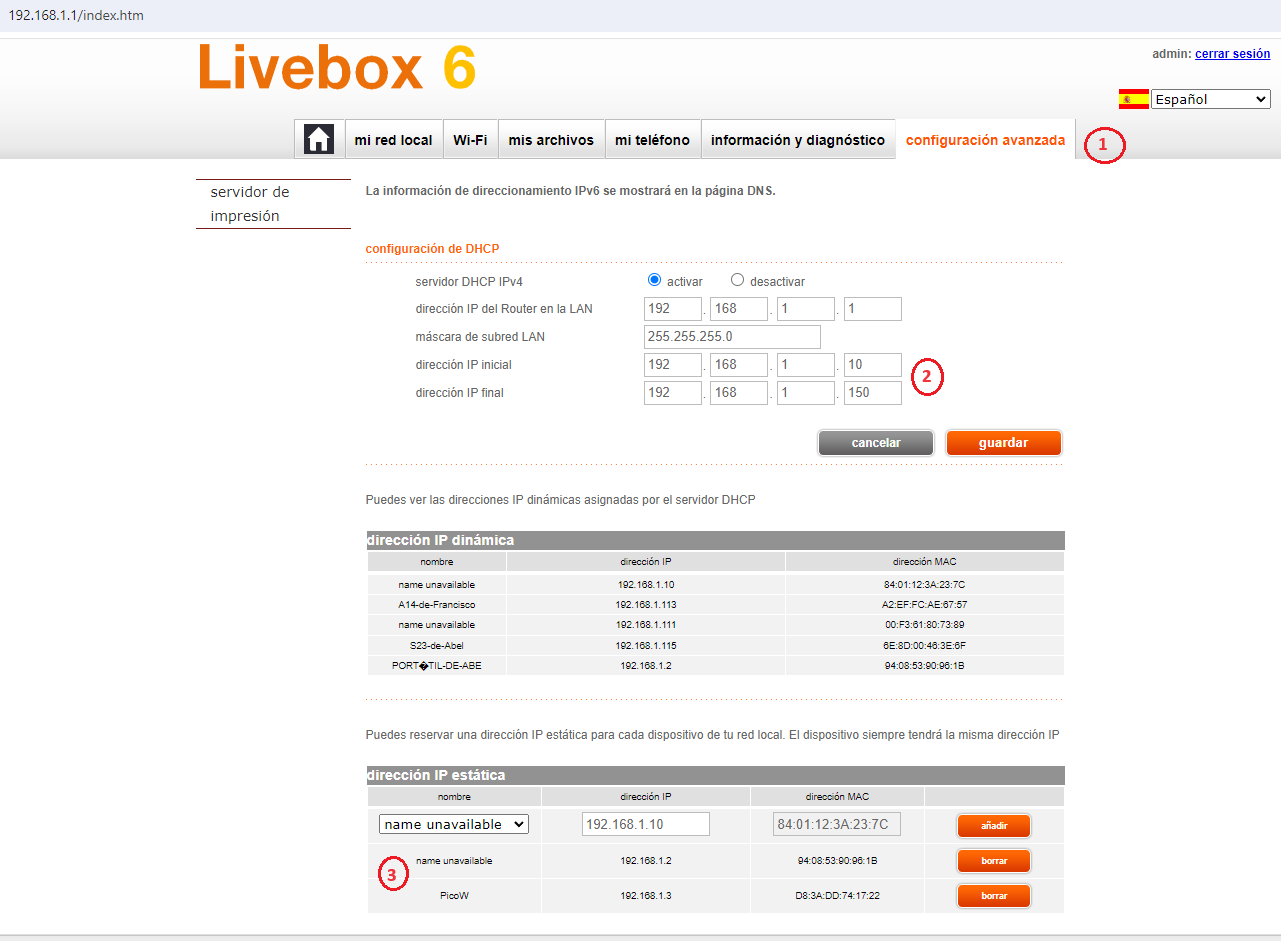
\includegraphics[width=1\linewidth]{../images/router_config.png}
	\caption{\label{fig:configuracion router}Configuración de red del router.}
\end{figure}

\subsection{Problema 2: Volumen Docker}
Para poder mantener los datos de la base de datos de manera persistente se debe crear un volumen de Docker.
Para ello en la aplicación Docker Desktop se accede a la opción de \texttt{``Volumes''} y se crea un volumen con el nombre \texttt{``database''} como se muestra en la figura \ref{fig:volumen docker}.
\begin{figure}[H]
    \raggedright
    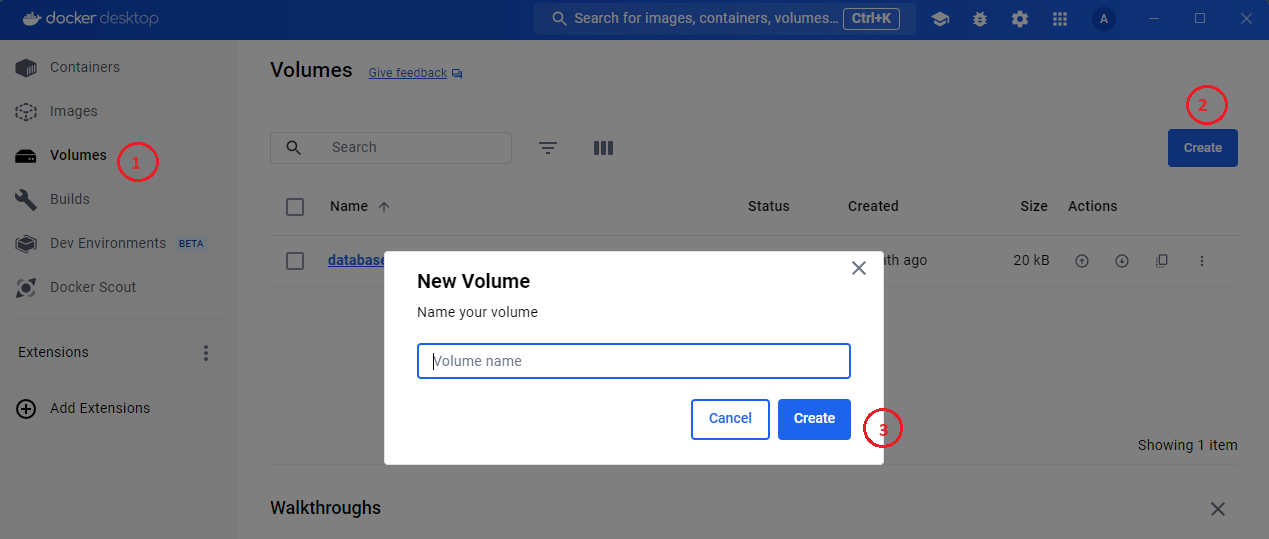
\includegraphics[width=1\linewidth]{../images/volumen_docker.png}
    \caption{\label{fig:volumen docker}Creación de un volumen de Docker.}
\end{figure}

Y se observa como en el archivo \texttt{``build.bat''} se enlaza el volumen con el contenedor mediante el comando \texttt{``-v database:/home/database''}.


\subsection{Problema 3: Envío de datos a Ubidots}
Para poder enviar los datos a Ubidots se debe configurar el dispositivo en Ubidots y obtener el token de la API.
El token de la API se debe enviar en la cabecera de la petición HTTP.
Para ello se debe buscar en la \href{https://docs.ubidots.com/reference/authentication}{documentación de Ubidots} el formato de la petición y enviar los datos en el formato correcto con la cabecera \texttt{``X-Auth-Token''}.
\begin{lstlisting}
def add_user_ubidots(uid):
    ...
    request = requests.post(
        URL_UBIDOTS,
        headers={'X-Auth-Token': TOKEN_UBIDOTS, 'Content-Type': 'application/json'},
        json=data
    )
    ...
\end{lstlisting}

\section{Resultados obtenidos}
Se ha logrado implementar un sistema de control de acceso mediante llaves y tarjetas RFID con un microcontrolador Raspberry Pi Pico WH y un servidor con una base de datos SQLite y una API REST.
Se ha logrado enviar los datos de registro de usuarios y accesos a Ubidots para su visualización en tiempo real.
Se ha logrado cambiar el modo de lectura de la llave o tarjeta RFID mediante Bluetooth Low Energy.
Se ha logrado encender un LED tricolor en función de la respuesta de la API.
La aplicación ha sido probada con éxito y se ha logrado registrar usuarios y accesos de manera correcta.\\
Como trabajo futuro se propone mejorar la seguridad del sistema mediante la encriptación de los datos y la escalabilidad del sistema con varias Raspberry Pi Pico WH y lectores RFID que se comuniquen con el servidor.
También se podría cambiar la tecnología de lectura de llaves y tarjetas RFID por NFC, un sistema de reconocimiento facial o de huella dactilar para mejorar la seguridad del sistema.

\addcontentsline{toc}{section}{Referencias} % Agregar la sección de Referencias al índice
\bibliographystyle{plain}
\bibliography{refs}



\end{document}
